\documentclass[a5paper,11pt]{article}

%----------Idioma---------
\usepackage[spanish]{babel}

%---------Margenes--------
\usepackage[right=2.5cm,left=3cm,top=2.5cm,bottom=2.5cm]{geometry}

%--------Para poner símbolos especiales----------
\usepackage[utf8]{inputenc}

%-------Simbolos----
\usepackage{bbding}

%----colores-----
\usepackage[dvipsnames,usenames,svgnames,x11names]{xcolor}

%-----Imágenes----
\usepackage{graphicx}

%----Caption----
\usepackage{caption}

%----Mover el caption o las leyendas-----
\usepackage[right]{sidecap}

%----Color del fondo de todas las páginas---
\pagecolor{brown}

%----Color de letra de todas las páginas---
\color{white}

%------------------------
\usepackage{fancyhdr}

%-------------------------
\pagestyle{fancy}

    \fancyhf{}
    \chead{Información sobre la serie} 
    \lfoot{Villa Rosas Esteban}
    \rfoot{\thepage}
    

\begin{document}
\begin{center}

{\Huge{{\textbf{\emph{\underline{Salvation}}}}}}\\

{\small{Esteban Villa Rosas }}\\

{\small{September 22, 2022}}

\end{center}

\section{\Large{\emph{Información sobre la serie}}}
    \subsection{\large{\underline{Reseña}}} \small{Pues, en primer lugar, esta es una serie que tiene como subgeneros a la {\textbf{\emph{\underline{Ciencia - Ficción}}}} y la  {\textbf{\emph{\underline{Intriga}}}}, pues en cualquier momento puedes estar tranquilamente disfrutando de la serie, y de repente estas ancioso por querer saber lo que viene, pues te deja en suspenso. Así mismo, la serie se sigue con interés y su visionado resulta agradable porque todo está revestido de cierta elegancia: los escenarios, el vestuario y la utilería en general y los protagonistas. 
    
    Por otra parte, para entrar un poco en contexto con la serie, podemos decir que en general trata sobre; un estudiante graduado del MIT, Liam Cole y el multimillonario técnologo, Darius Tanzs, quienes descubren que un asteroide está a solo seis meses de colisionar en la tierra. Con toda la delicadeza y sin crear un escándalo público comienzan a trabajar juntos en un plan para salvar a la humanidad. Para ello, reclutan a una chica que soñaba ser escritora, Jillian, para dar el enfoque teórico al planteamiento. Pero dentro de la dificultad, la cosa se complica con la entrada del gobierno. Ambos se ponen en contacto con Grace Barrows, oficial del Pentagono, que se verá envuelta en un caos y se ve en la necesidad de prestar atención a ambos lados. Ya que el gobierno le da otro enfoque y Harris Edwards, Secretario Adjunto de Defensa, es el encargado de ejecutar un plan secreto de ataque para desviar el asteroide.
    
    Dicho lo anterior, lo que sorprende y engancha de ``Salvation'' es la mezcla de géneros: partiendo de una catástrofe espacial que amenaza con la destrucción del planeta va girando hacia la intriga política con la Casa Blanca como centro de las luchas por el poder económico mundial.
    
    Esta amplia cifra de temas hace a ``Salvation'', como digo, un título atractivo para un público amplio en cuanto a gustos, pero también en ello se encuentran las objeciones, ya que ``el que mucho abarca poco aprieta'' y al final todas las líneas abiertas
    se desarrollan con bastante profundidad y facilidad.
    
    Por último, me parece que ``Salvation" solo tiene dos temporadas, ya pesar de que la última escena del último capítulo deja sensación de querer más, la serie queda suficiente y satisfactoriamente concluida.}
    
    \subsection{\large{\underline{Elenco de actores}}} \small{
    \setlength{\parindent}{0pt}\HandRight\textbf{ Directores}
    
\begin{enumerate}
    
    \item Stuart Gillard
    \item Maja Vrvilo
    \item Kenneth Fink
    \item Robert Duncan McNeill
    \item Greg Beeman
    \item Jennifer Lynch
    \item Juan Carlos Fresnadillo
    \item Edward Ornelas
    \item Dan Lerner
    \item Nick Gomez
    \item Russell Lee Fine
    
\end{enumerate}  

    \setlength{\parindent}{0pt}\HandRight\textbf{ Personajes/Actores principales}
    
\begin{enumerate}
    \item Darius Tanz - Santiago Cabrera
    \item Grace Barrows - Jennifer Finnigan
    \item Liam Cole - Charlie Rowe
    \item Jillian Hayes - Jacqueline Byers
    \item Zoe Barrows - Rachel Drance
    \item Amanda Neel - Shazi Raja 
    \item Harris Edwards - Ian Anthony Dale
    \item Alonzo Carter - Ashley Thomas 
    \item Alycia Vrettou - Melia Kreiling
    
\end{enumerate}  


    \setlength{\parindent}{0pt}\HandRight\textbf{ Personajes/Actores Secundarios}

\begin{enumerate}

     \item Malcolm Croft - Dennis Boutsikaris
     \item Claire Rayburn - Erica Luttrell
     \item Pauline Mackenzie - Tovah Feldshuh
     \item Karissa - Josette Jorge 
     \item Monroe Bennett - Sasha Roiz
     \item Hugh Keating - Mark Moses 
     \item Randall Calhoun - Brian Markinson
     \item Daniel Hayes - Jeffrey Nordling
     \item Nicholas Tanz - John Noble 
     \item Theresa/Tess - Autumn Reeser
     \item Dylan Edwards - André Dae Kim 
     \item Dra. Rosetta Stendahl - Anjali Jay 
     \item Dr. Chandra - Manoj Sood 

\end{enumerate}    

    \setlength{\parindent}{0pt}\HandRight\textbf{ Guionistas}

\begin{enumerate}

     \item Mike Werb
     \item Blake Taylor
     \item Elizabeth Kruger
     \item Craig Shapiro

\end{enumerate}    
    }
    
    \subsection{\large{\underline{Descripción de los personajes}}} \small{
    
\begin{itemize}

     \item[\Plane]\fcolorbox{black}{blue}{\textcolor{yellow}{Darius Tanz:}} Un científico multimillonario que es el fundador y director ejecutivo de Tanz Industries y un jugador fundamental en la defensa de los Estados Unidos contra el inminente asteroide. Darius se desempeña brevemente como vicepresidente de los Estados Unidos antes de convertirse en presidente después del asesinato del presidente Mackenzie.
     \item[\Plane] Malcolm Croft: Profesor del MIT y mentor de Liam.
     \item[\Plane]\fcolorbox{black}{pink}{\textcolor{blue}{Grace Barrows:}} La secretaria de prensa del Pentágono , luego asesora principal del presidente Mackenzie y más tarde del presidente Tanz; tiene una relación íntima con Harris Edwards, subsecretario y, más tarde, secretario de Defensa, y trabaja con Darius para evitar la colisión del asteroide.
     \item[\Plane]  Claire Rayburn: Asesora principal y más tarde jefa de personal de la Casa Blanca del presidente Monroe Bennett.
     \item[\Plane]\fcolorbox{black}{green}{\textcolor{orange}{ Liam Cole:}} Estudiante del MIT y más tarde protegido de Darius; es una de las primeras personas fuera del gobierno en predecir la inminente colisión del asteroide con la Tierra. Él y Darius trabajan juntos en un motor EM para un tractor de gravedad que esperan usar para cambiar el curso del asteroide.
     \item[\Plane] Pauline Mackenzie: La presidenta de los Estados Unidos.
     \item[\Plane]\fcolorbox{black}{red}{\textcolor{green}{Jillian Hayes:}} Una escritora de ciencia ficción de Boston que se involucra con Liam y luego es elegida por Darius para elegir a 160 supervivientes que abandonen la Tierra si no se puede detener la colisión de asteroides.
     \item[\Plane] Karissa: Asistente de Darius.
     \item[\Plane]\fcolorbox{black}{yellow}{\textcolor{blue}{Zoe Barrows:}} Hija de Grace.
     \item[\Plane] Monroe Bennett: La vicepresidenta y más tarde presidenta de los Estados Unidos.
     \item[\Plane]\fcolorbox{black}{violet}{\textcolor{green}{Amanda Neel:}} Una reportera de investigación que busca la verdad sobre los secretos de Darius y del gobierno. Después de enterarse del asteroide, Amanda es asesinada antes de que pueda publicar la historia.
     \item[\Plane] Hugh Keating: Padre de Grace y ex agente de la CIA
     \item[\Plane]\fcolorbox{black}{orange}{\textcolor{blue}{Harris Edwards:}} Un graduado de la Academia de la Fuerza Aérea de los Estados Unidos que ahora se desempeña como Subsecretario de Defensa de los Estados Unidos y es una de las pocas personas en Washington, DC que conoce el impacto inminente del asteroide. Se le describe como un operativo habilidoso, pero un burócrata aún mejor. Después de que su superior es despedido, es ascendido a Secretario de Defensa .
     \item[\Plane] Randall Calhoun: El Secretario de Defensa de los Estados Unidos que luego es despedido por el presidente Mackenzie y reemplazado por Harris Edwards.
     \item[\Plane]\fcolorbox{black}{purple}{\textcolor{yellow}{Alonzo Carter:}} Un detective de la policía de DC que investiga la desaparición de Claire Rayburn.
     \item[\Plane] Daniel Hayes: Padre de Jillian y librero.
     \item[\Plane]\fcolorbox{black}{gray}{\textcolor{purple}{Alycia Vrettou:}} Una brillante científica informática, ex protegida de Darius Tanz y miembro de RE / SYST, liderando un grupo internacional de científicos cautivos para idear un plan para prevenir la colisión de asteroides.
     \item[\Plane] Nicholas Tanz: Tío de Darius y presidente de la junta directiva de Tanz Industries.
     \item[\Plane] Theresa: También conocida como Tess, el primer amor de Darius.
     \item[\Plane] Dylan Edwards: Hijo de Harris y miembro de la organización de hackers RE / SYST.
     \item[\Plane]  Dra. Rosetta Stendahl: Una vieja amiga de Darius y una científica brillante. Se une a Darius y lidera el proyecto para preparar un cañón de riel destinado a ayudar a desviar el asteroide.
     \item[\Plane] Dr. Chandra: Un especialista internacional en Dinámica Orbital y Teoría General de la Purturbación.
    
\end{itemize}

    }

\begin{SCfigure}
    
    \begin{flushright}
    \caption*{Salvation - Serie }
    
\includegraphics[scale=0.40,angle=15]{salvation.jpg}
    \end{flushright}
\end{SCfigure}    

\pagestyle{fancy}

    \fancyhf{}
    \chead{Razones por las que elegí esta serie} 
    \lfoot{Villa Rosas Esteban}
    \rfoot{\thepage}
    
\section{\Large{\emph{Razones por las que elegí esta serie}}}
    \subsection{\large{\underline{Gobierno}}} \small{\textcolor{green}{En principio, y creo que es lo más importante, del por qué elegí esta serie, es porque, al terminarla de ver, me di cuenta, no solo que me gustaba mucho la ciencia ficción y la intriga, sino que también por la manera en que esta serie te permite ver, cómo es que {\textbf{\emph{\underline{los gobiernos  pueden manipular}}}} fuertemente a la sociedad, aquí lo podemos ver, nadie supo de que el asteroide colisionaría con la tierra durante meses, hasta que se tuvo que decir, entonces, tal ves en este preciso momento puedan estar los gobiernos planteando ideas o ideando como enfrentar algún problema, que nosotros ni siquiera sabemos que existe, esto fué una de las principales razones las que me gusta está serie y por lo que la elegí.}}
    
    \subsection{\large{\underline{Imaginación}}} \small{\textcolor{purple}{Así mismo, otra de las razones por las que me gusta esta serie es porqué he disfrutado mucho , aparte de que me reí por ciertas cosas, me facina y me encanta precisamente que no sea todo tan científicamente correcto y que deje lugar a la {\textbf{\emph{\underline{imaginación}}}}, es decir a la {\textbf{\emph{\underline{ficción}}}}.}}
    
    \subsection{\large{\underline{Perdidas emocionales y sociales}}} \small{\textcolor{yellow}{Por último, me gustaría mencionar que algo que amé de esta serie, es el caos y el alivio, pues después, de pelear, sufrir, días y noches sin dormir, muertes, explosiones, llegan a la conclusión de que no era un asteroide lo que chocaría con la tierra, y  por lo que tanto tiempo habían dado, sino que era como un colibrí, que avanzaba y retrocedía, siguiendo un patrón, y que por lo cual no había estallado contra la tierra. Pero retomando la idea, digo que me facina el {\textbf{\emph{\underline{caos}}}} y el {\textbf{\emph{\underline{alivio}}}} de la serie, ya que
    después de todo esto, todo de tranquiliza a lo máximo, ya no hay estrés, ya no hay peleas, las parejas destruidas tratan de reconciliarse, por qué aunque no lo creamos, al estar trabajando en un proyecto o el estar investigando, todo te molesta, y no quieres que te interrumpan, por lo que pierdes vida social, y a veces a tu pareja o hasta tu familia.}}
    
\hspace{-3.5cm} ``La vida está 

\hspace{-3.5cm}llena de

\hspace{-3.5cm}posibilidades. 

\hspace{-3.5cm}No hay mañana

\hspace{-3.5cm}sin nosotros.''

\newpage{}
\begin{SCfigure}

    \begin{flushright}
    \caption{Liam Cole, Estudiante del MIT. }
    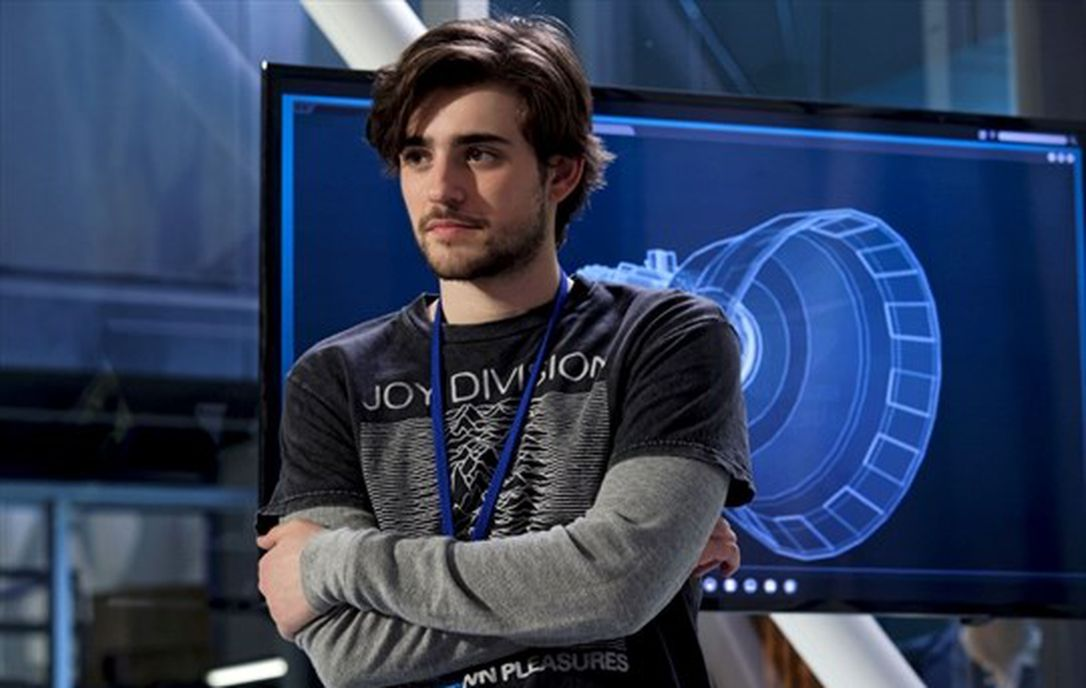
\includegraphics[angle=-18,width=6cm,height=3cm]{Liam.jpg}
    \end{flushright}
\end{SCfigure}

\begin{SCfigure}

    \begin{flushright}
    \caption{Nicholas Tanz, tío de Darius y presidente de la junta
directiva de Tanz Industries.}
    
\includegraphics[angle=8,width=5cm,height=5cm]{Nic.jpg}
    \end{flushright}
\end{SCfigure} 

\end{document}

